
% ----------------------------------------------------------------------
\introduction
\label{sec:intro}
% ----------------------------------------------------------------------

The numerical modelling of past glaciers and ice sheets allows indirect confrontation between glaciological theories and geomorphological reconstructions, challenging the validity of both. Yet a major obstacle in this exercise resides in the large uncertainties that affect climate forcing of numerical glacier models \citep{hebeler-etal-2008}. This includes the uncertainty on Earth's present climate, and the larger uncertainty on its changes in the past.

Our area of focus for the present study is the Cordilleran Ice Sheet in north-western North America. In a numerical modelling perspective, it is one of the least studied paleo-ice sheets on Earth, where nethertheless significant geomorphological data is available \citep{jackson-clague-1991}.
The Cordilleran Ice Sheet has been previously modelled as part of the North American ice sheet complex \citep{marshall-clarke-1999,calov-etal-2002,tarasov-peltier-2004,bintanja-etal-2005,gregoire-etal-2012} and within a larger-scale Arctic or Global numerical domain \citep{huybrechts-tsiobbel-1996,charbit-etal-2002,johnson-fastook-2002,zweck-huybrechts-2005,abeouchi-etal-2007,charbit-etal-2013}. In those studies, various climate forcing methods have been used, ranging from simplistic parametrizations to coupling to General Circulation Models (GCM).

\begin{itemize}

  \item \citet{johnson-fastook-2002} used a parametrized climate forcing based on elevation and distance from a climatic pole initiallly developped for Antarctica \citep{fastook-prentice-1994}.

  \item \citet{bintanja-etal-2005} used present-day reanalysis data as a reference climate to which they applied time-dependant temperature offsets to recreate glacial conditions. While this method ensures a more accurate representation of present climate, the approach to past climate change remain simplistic.

  \item \citet{huybrechts-tsiobbel-1996} use GCM output from a palæo-climate simulation to force an ice-sheet model to steady-state. Due to GCMs' computational expense, palæo-climate simulations were typically run for discrete ages of reasonably known ice-sheet configuration, such as the LGM. To produce time-dependant climate forcing, glacier modellers interpolated GCM output in time between different simulations, either linearly \citep{charbit-etal-2002} or more commonly using a wieghting function based on ice-core records \citep{marshall-clarke-1999,tarasov-peltier-2004,zweck-huybrechts-2005,gregoire-etal-2012}. GCM palæo-climate simulations typically rely on ice-sheet reconstructions of the type of ICE-4G \citep{peltier-1994} for their surface topography boundary condition. In turn, ice-sheet models based on these simulations generally reproduce LGM ice extents closely consistent with the reconstruction.

  \item Finally \citet{yoshimori-etal-2001,calov-etal-2002,abeouchi-etal-2007,charbit-etal-2013} couple their ice-sheet models to GCM of coarser resolution and reduced complexity.

\end{itemize}

%TODO tarasov-peltier-1997

If these studies reproduce well the magnitude of the North American glaciation at Last Glacial Maximum, there is a general tendency for studies that do not undirectly rely on reconstructions of the type of ICE-4G\citep{johnson-fastook-2002,bintanja-etal-2005,huybrechts-tsiobbel-1996,charbit-etal-2002,marshall-clarke-1999,tarasov-peltier-2004,zweck-huybrechts-2005,gregoire-etal-2012}  to predict excessive ice cover in northern Yukon Territory and Alaska, regions that have not been covered by ice in hundreds of thousands of years \citep{dukrodkin-1999,kaufman-manley-2004}.

Here we use a Parallel Ice Sheet Model (PISM) \citep{web:pism} to simulate the entire Cordilleran Ice Sheet at the Last Glacial Maximum (LGM). We force our model with multiple climate datasets and compare our results to the mapped LGM ice sheet margin from \citet{kleman-etal-2010}. See \citet{quiquet-etal-2012} for a similar comparison on Greenland. To avoid circular dependance on prescribed ice sheet geometries, and allow high spatial resolution in our climate forcing, we use present-day climate data and given temperature offsets in a manner similar to \citet{bintanja-etal-2005}. To our knowledge, this is the first modelling study which specifically focus on the Cordilleran Ice Sheet since the one by \citep{robert-1991}, who focused specifically on its southern margin.

\begin{figure}[t]
	\vspace*{2mm}
	\begin{center}
		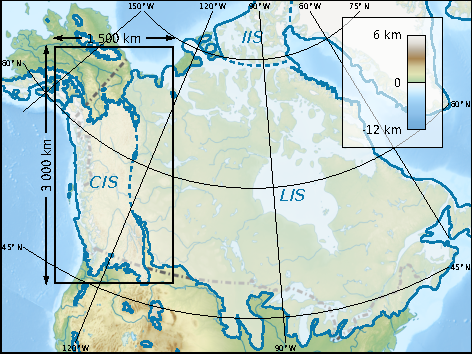
\includegraphics[width=8cm]{cordillera-climate-locmap}
	\end{center}
	\caption{Shaded relief map of northern North America. The frame delimits this study's modelling domain. The outlines of the former ice sheets are from \citet{kleman-etal-2010}. The background map was made with ETOPO1 \citep{data:etopo1} and Natural Earth Data \citep{data:naturalearth}.}
	\label{fig:locmap}
\end{figure}

